This experiment originates in McKenzie \etal (1974) \cite{mcrw74}. The domain is a 2D 
square of size $L$. The fluid is incompressible, and the Boussinesq approximation is used.
Boundary conditions are free slip on all sides. $T=0$ is prescribed at the bottom 
and $T(x)=T_0 \cos (\pi x/L)$ at the top. The two sides are insulated.

Following Sato \& Thompson (1976) \cite{sath76}, 
parameters are $\kappa=1.5\cdot 10^{-6}\si{\square\m\per\second}$, 
$\rho_0=3700\si{\kg\per\cubic\metre}$, $\alpha=2\cdot 10^{-5}\si{\kelvin}^{-1}$, 
$\eta=2\cdot10^{17} \rho_0 = 7.4\cdot10^{20} \si{\pascal\second}$, $g=10\si{\metre\per\square\second}$, 
$C_p=1200 \si{\joule\per\kg\per\kelvin}$, $T_0=0.1,1,10\si{\kelvin}$.  

We then deduce that $k=\kappa \rho_0 C_p = 6.66$. The Rayleigh number is given by
\[
\Ranb = \frac{ \rho_0 g \alpha T_0 L^3  }{\kappa \eta}
\]
In the paper three values $\Ranb=45.8,158,4580$ are used  corresponding to $T_0=0.1,1,10$. 
However there is a problem since then 
\[
L = \left( \frac{\Ranb \kappa \eta}{\rho_0 g \alpha } T_0   \right)^{1/3}
= \left( \frac{458\cdot 1.5e-6\cdot 7.4e20}{3700\cdot 10\cdot 2e-5 } 1   \right)^{1/3}
= \left( 6.87e17 \right)^{1/3}
\simeq 882.361 \si{\kilo\metre}
\]
and the vertical dimension of the box is given in \cite{mcrw74} as 700\si{\km}. 
We then find that there is effectively a factor 2 missing in the Rayleigh number in order
to reconcile the above parameters with the desired Rayleigh numbers... 
Given how very plausible $\kappa$, $C_p$, $\alpha$ and $\rho_0$ are, I choose to 
decrease the viscosity by a factor two.
We then have 
\[
\{ 45.733, 457.33, 4573.3 \} = \frac{ \rho_0 g \alpha  L^3  }{\kappa \eta} \{ 0.1, 1 , 10\}
\]

\begin{center}
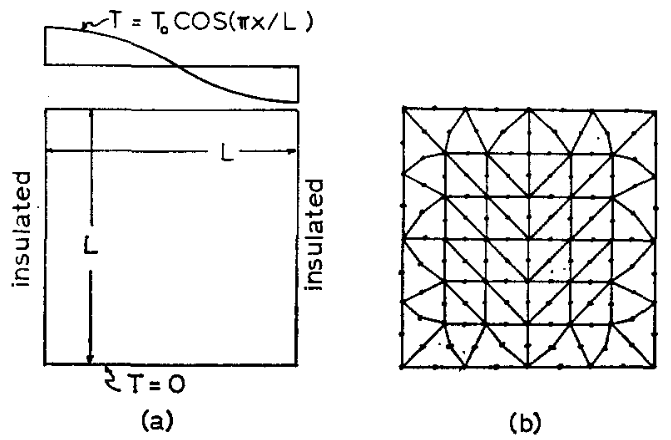
\includegraphics[width=6cm]{python_codes/fieldstone_38/images/sath76_a}
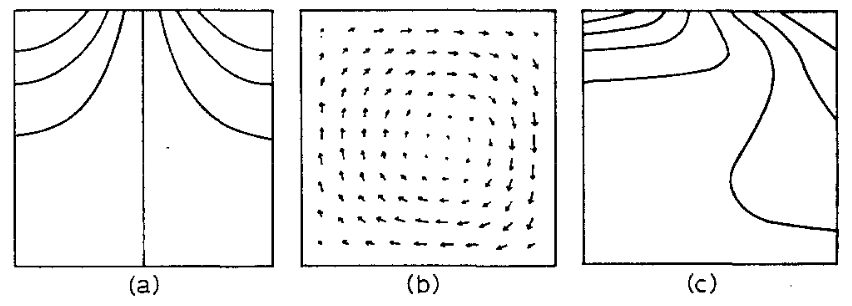
\includegraphics[width=8cm]{python_codes/fieldstone_38/images/sath76_b}\\
{\captionfont Left: (a) Boundary conditions; (b) Mesh layout - the authors
use $P_2\times P_1$ elements;\\
Right: Isotherms and velocity field: (a) Steady-state conduction;
velocity field; (c) Steady-state isotherms R = 4580.}
\end{center}

The code is based on \stone~03, and because velocities are very small for low Rayleigh numbers
reduced densities are used, i.e. the buoyancy force in the Stokes equation is given by $-\alpha(T-T_0)\vec{g}$.
Steady state is reached when the velocity and temperature fields do not change by more than $tol=10^{-6}$.


As explained in McKenzie \etal (1974), for $\Ranb <<1$ advection of heat is negligible and $T$ is therefore harmonic:
\[
T(x,y) = \Delta T \cos (\pi x/L) \frac{\sinh \pi z/L}{\sinh \pi L_y/L_x}
\]


\begin{center}
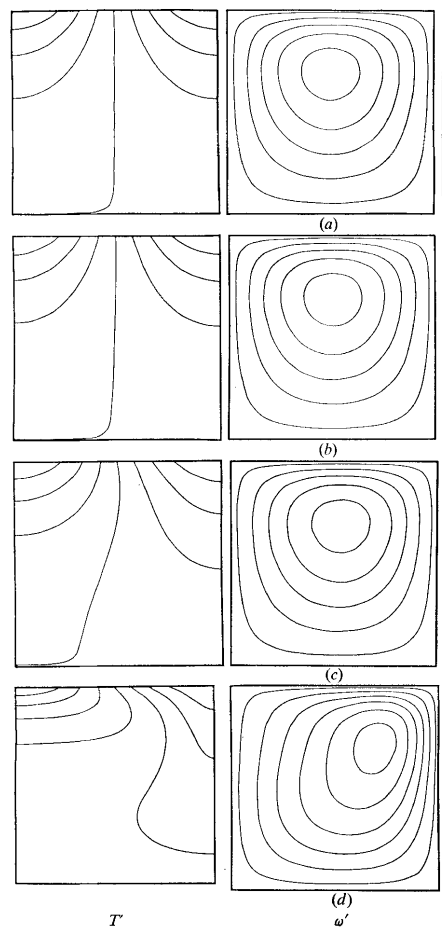
\includegraphics[width=6cm]{python_codes/fieldstone_38/images/mcrw74}\\
{\captionfont Temperature isocontours are uniformly spaced with interval $T_0/4$.
a-d: $T_0=0.01,0.1,1,10$}
\end{center}



